\documentclass{beamer}[UTF-8]
\usepackage{ctex}
\usepackage{graphicx}
\usepackage{listings}
\usepackage{fontspec}
\setmonofont{Fira Code}
\usetheme{CambridgeUS}
\setCJKsansfont{SimSun}

\title{Lesson 2——搜索}
\subtitle{NOIP非基础新课}
\author{Garen Wang}
\date{\today}

\begin{document}
\maketitle
\begin{frame}{目录}
搜索可以讲得很难,但是我讲不来。所以大概就是下面这些:  \pause
\tableofcontents
\end{frame}

\section{回溯思想和bfs}

\begin{frame}{回溯思想(backtracking)}
  \pause
\begin{itemize}
  \item 利用递归搞的搜索大多都要用到这种回溯思想。 \pause
  \item 回溯法采用试错的思想,它尝试分步的去解决一个问题。 \pause
  \item 在分步解决问题的过程中,当它通过尝试发现现有的分步答案不能得到有效的正确的解答的时候,它将取消上一步甚至是上几步的计算,再通过其它的可能的分步解答再次尝试寻找问题的答案。 \pause
  \item 具体实现的样子就是: \pause
  \item 进入新一步,修改相应状态;退出一步,把之前改过的改回来,走其他的路。
\end{itemize}
\end{frame}

\begin{frame}[fragile]{回溯框架}
\begin{lstlisting}[language = C++,
numberstyle=\tiny,keywordstyle=\color{blue!70},
commentstyle=\color{red!50!green!50!blue!50},frame=shadowbox,
rulesepcolor=\color{red!20!green!20!blue!20},basicstyle=\ttfamily]
void dfs(int t, 其他需要的参数) {
    if(t > n) {
        if(满足条件) 输出;
        return;
    }
    for(int i = start; i <= end; i++) {
        if(满足能选的条件) {
            做标记;
            dfs(t + 1, 其他需要的参数);
            把标记改回来;
        }
    }
}
\end{lstlisting}
\end{frame}

\begin{frame}{例题:八皇后问题}
  \pause
\begin{itemize}
\item 给你8*8的方格,放8个皇后,让皇后们不能互相攻击,即不能处于同一行、同一列或同一对角线。 \pause
\item 利用回溯法,在第𝑘行放皇后视为第𝑘步,行中的每一个点都去判断是否合法,若合法即放置皇后进入下一步。 \pause
\item 同样,进入下一步涉及到标记的修改和改回来两个操作。 \pause
\item 八皇后问题用回溯法解决还没什么大问题,因为回溯法不加剪枝最坏是有指数级的复杂度。 \pause
\item 八皇后的扩展:n皇后问题。有一种二进制的方法可以快速解决。这里就不讲了。
\end{itemize}
\end{frame}

\begin{frame}{dfs(深度优先搜索)}
  \pause
\begin{itemize}
\item 在树的遍历中有三种深度优先的遍历,同理也有深度优先的搜索。 \pause
\item 在寻找连通块的过程中,经常使用到dfs。这时有一种称呼:floodfill(洪水填充)。 \pause
\item 回溯法就是使用dfs的框架。 \pause
\item dfs相信大家都学过,就不细讲了。
\end{itemize}
\end{frame}

\begin{frame}{例题1:luoguP1312}
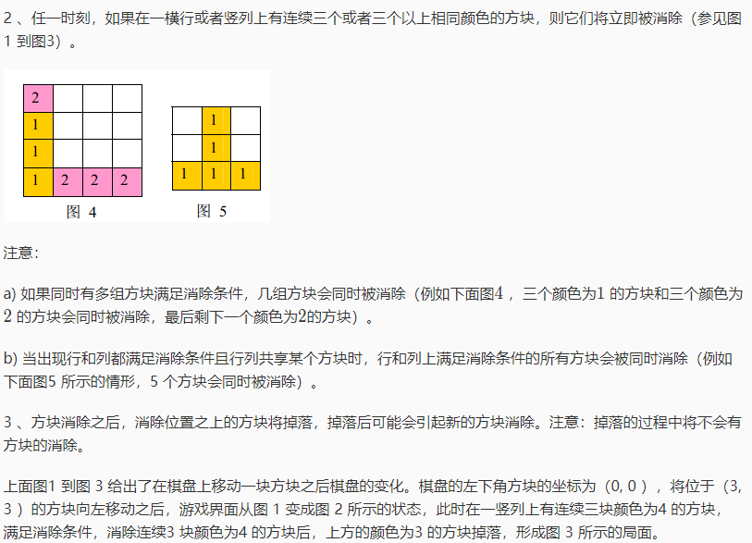
\includegraphics[width=\textwidth, height=\textheight]{temp1.png}
\end{frame}

\begin{frame}{例题1:luoguP1312}
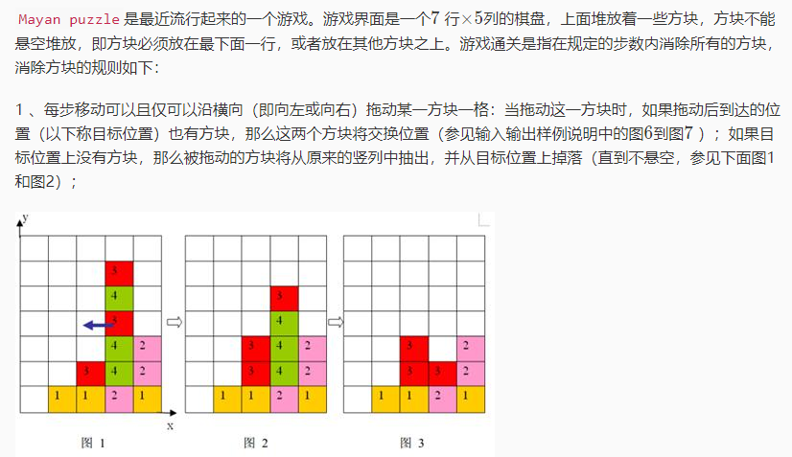
\includegraphics{temp2.png}
\end{frame}

\begin{frame}{例题1——分析}
  \pause
\begin{itemize}
\item 这道题就是一道大模拟题,主要考察dfs搜索框架、剪枝和码力。 \pause
\item 因为搜索步数只有5,所以直接用dfs就行了。 \pause
\item 搜索的每一步就是枚举一个方块,与左右交换,同时增加一步。 \pause
\item 其实这道题最重要的就是如何处理方块掉落和方块消除。 \pause
\item 方块掉落:枚举每一列,从下往上遍历,记录当前遍历到的空格数,用老方块迭代掉新方块。 \pause
\item 方块消除:弄一个vis数组,枚举所有方块,用一个if确定至少的3个,然后左右或者上下扩展。
\end{itemize}
\end{frame}

\begin{frame}{例题1——分析}
  \pause
\begin{itemize}
\item 但是你以为这样就完了? \pause
\item 其实还需要剪枝。 \pause
\item 这里有两个剪枝: \pause
\begin{enumerate}
  \item 交换两个相同的方块时,剪枝! \pause
  \item 若一个方块向左交换另一个方块时,剪枝!(因为从另一个方块向右交换过来会更优) \pause
\end{enumerate}
\end{itemize}
然后就完事了。
\end{frame}

\begin{frame}{例题2:luoguP2668}
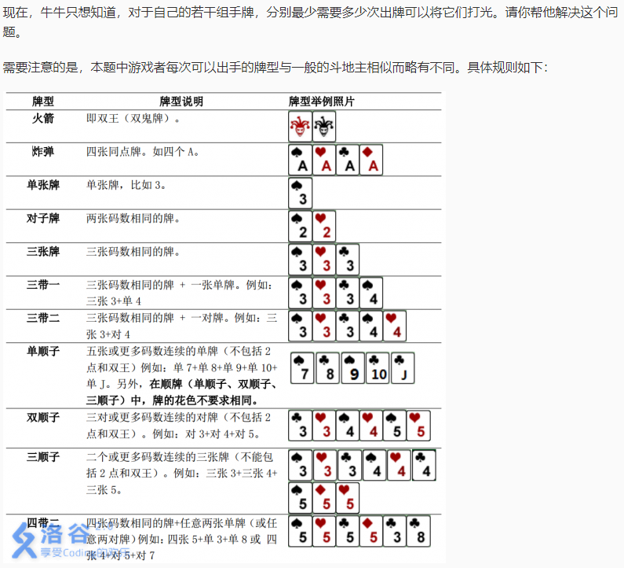
\includegraphics[width=\textwidth, height=\textheight]{luoguP2668.png}
\end{frame}

\begin{frame}{例题2——分析}
  \pause
\begin{itemize}
\item 同样是个大模拟。 \pause
\item 我们用桶把所有的牌都存下来。之后的所有操作都建立在桶上。 \pause
\item 因为题意里面与花色一点关系都没有,所以直接抛弃掉这个信息。 \pause
\item 考虑你玩斗地主的做法:先出带牌和顺子,再出对子和单牌。 \pause
\item 打到最后的单牌是没必要回溯的,是可以直接看出答案的。 \pause
\item 所以程序的思路就出来了:先暴力枚高级牌,再贪心打低级牌。
\end{itemize}
\end{frame}

\begin{frame}{例题2——分析}
  \pause
\begin{itemize}
\item 所以那个dfs函数的思路就可以出来了: \pause
\begin{enumerate}
  \item 考虑四带两对、四带两张单牌、炸弹、三带一对、三带一张单牌、三张牌。 \pause
  \item 考虑三顺子、双顺子、单顺子。 \pause
  \item 最后遍历所有的牌,剩一张就单张牌,剩两张就出对。 \pause
\end{enumerate}
\item 注意:火箭在这里没什么卵用,只需要看成一种对子就可以。 \pause
\item 因为求的是最少次数,也可以适当性来一点最优性剪枝。 \pause
\item 因为$n \leq 23$,实际上搜一组数据也并不会太慢。
\end{itemize}
\end{frame}

\begin{frame}{作业}
\begin{itemize}
  \item luogu试炼场pj组的“深度优先搜索”专题做到绿。
  \item luoguP1784 数独(后面会用到)
\end{itemize}
\end{frame}

\section{bfs}

\begin{frame}{bfs(广度优先搜索)}
  \pause
\begin{itemize}
  \item 树是有层次遍历的,就叫bfs。在搜索上也有类似的bfs。 \pause
  \item bfs需要使用队列实现,每次取出队头,进行扩展,扩展出的新节点在队尾进入。 \pause
  \item 给一个例子理解一下:
\end{itemize}
\end{frame}

\begin{frame}[fragile]{bfs框架}
\begin{lstlisting}[language = C++,
numberstyle=\tiny,keywordstyle=\color{blue!70},
commentstyle=\color{red!50!green!50!blue!50},frame=shadowbox,
rulesepcolor=\color{red!20!green!20!blue!20},basicstyle=\ttfamily]
void bfs(起点) {
    std::queue<类型> q;
    q.push(起点); vis[起点] = true;
    while(!q.empty()) {
        类型 x = q.front(); q.pop();
        for(扩展新节点) {
            if(!vis[新节点]) {
                q.push(新节点);
                vis[新节点] = true;
           }
        }
    }
}
\end{lstlisting}
\end{frame}

\begin{frame}{例题1:luoguP3956}
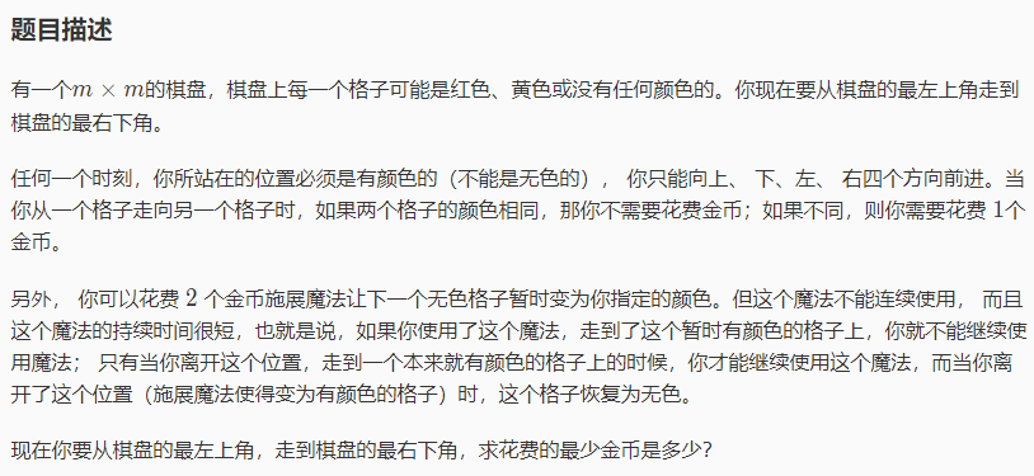
\includegraphics[width=\textwidth, height=\textheight]{luoguP3956.png}
\end{frame}

\begin{frame}{例题1——分析}
  \pause
\begin{itemize}
\item 一看就知道要用bfs嘛。用dfs可能会爆栈。 \pause
\item 利用bfs的一个优良性质:当第一次遍历到某节点时,即是最优。 \pause
\item 所以我们从(1,1)初始状态开始bfs,直到到达$(m,m)$为止,第一次搜到$(m,m)$即是最少的金币数。 \pause
\item 状态相比于普通bfs只需要再来一个bool:判断是否用了膜法。 \pause
\item 状态向四个方向转移,若颜色相同无需代价,若颜色不同需1块。 \pause
\item 当现在踩着的不是用膜法变的时,可以考虑花2块变色并踩上去。 \pause
\item 这就是最朴素的bfs思路。
\end{itemize}
\end{frame}

\begin{frame}{例题1——分析}
  \pause
\begin{itemize}
\item 你以为这样就能过了?Too young! \pause
\item 由于状态巨大,并且可能跑回去,实际上朴素bfs是有很大浪费的。 \pause
\item 我们可以记录一个dist数组,记录这种状态下最小金币花费。 \pause
\item 当转移后金币花费比最小金币花费还要贵的时候,不转移。只转移那些可能更优的状态。 \pause
\item 给大家看看代码。
\end{itemize}
\end{frame}

\begin{frame}{作业}
\begin{itemize}
  \item 把luogu试炼场pj组“广度优先搜索”做绿。
\end{itemize}
\end{frame}

\section{剪枝}

\begin{frame}{剪枝}
  \pause
\begin{itemize}
\item 普通的搜索人人都会写,但是写出来的不一定跑得过。 \pause
\item 在搜索的过程中可能会出现冗余状态,我们可以想办法删去。 \pause
\item 这种把搜索中的冗余状态消除掉的做法,叫做剪枝(prune)。 \pause
\item 剪枝是一项高级的运用,下面通过很多例题来了解一下。
\end{itemize}
\end{frame}

\begin{frame}{例题1:luoguP1433}
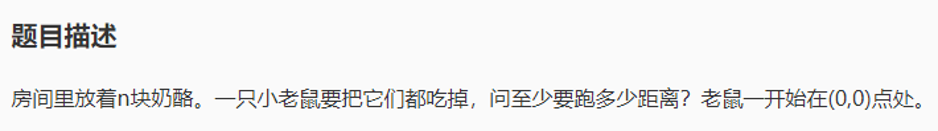
\includegraphics[width=\textwidth]{luoguP1433.png}
\end{frame}

\begin{frame}{例题1——分析}
  \pause
\begin{itemize}
  \item 震惊!堂堂TSP问题沦落为普及-! \pause
  \item 如果用搜索的思路,就是一个回溯的问题了。 \pause
  \item 自信地交上去,T了4个点。 \pause
  \item 在这里介绍第一种剪枝:最优性剪枝。 \pause
  \item 题目如果让你求最优答案,则大部分可以使用最优性剪枝: \pause
  \item 如果当前的中途答案比当前最优解还要劣,那么剪枝。 \pause
  \item 具体在这道题,直接一行代码搞定。 \pause
  \item 听说是可以用模拟退火的,但是我写没过。
\end{itemize}
\end{frame}


\begin{frame}{例题2:luoguP1731}
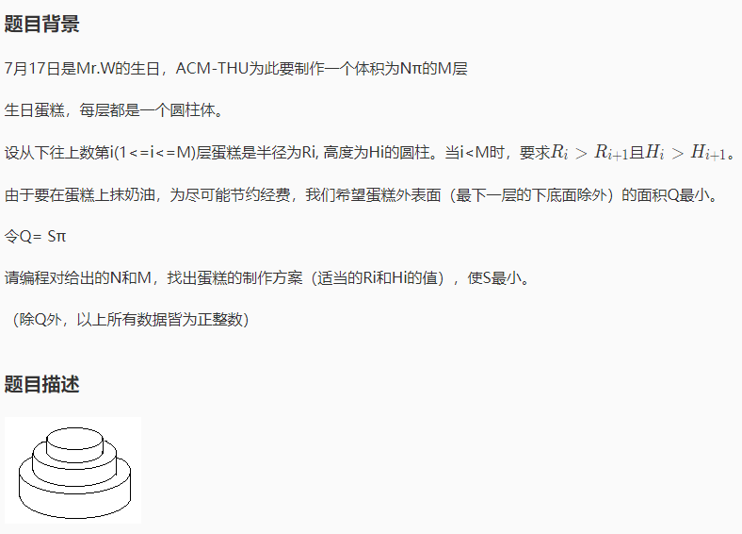
\includegraphics[width=\textwidth, height=\textheight]{luoguP1731.png}
\end{frame}

\begin{frame}{例题2——分析}
  \pause
\begin{itemize}
  \item 爆搜的思路确实很好想,但是不敢想:状态太多了! \pause
  \item 结合前面的最优性剪枝,这里在介绍另外一种剪枝:可行性剪枝。 \pause
  \item 当我们根据当前状态已经能够推断绝对不可能比当前最优解更优,则剪枝。这就是可行性剪枝。 \pause
  \item 参考这两个大方向,我们就有4个剪枝:
\end{itemize}
\end{frame}

\begin{frame}{例题2——分析}
  \pause
\begin{enumerate}
  \item 当前表面积比当前最小表面积大,剪枝。 \pause
  \item 当前表面积加上最少的表面积还比当前最小表面积大,剪枝。最少的表面积可以拿半径都是1的情况(虽然不可能实现)。 \pause
  \item 当前体积加上最大的体积还比$n$小,剪枝。当前最大的体积就是以当前的半径叠满为止(同样不可能实现,但不影响)。 \pause
  \item 把那些体积大于$n$、叠$m+1$层等非法情况掐掉。 \pause
  \item 最后就能过了。。。
\end{enumerate}
\end{frame}

\begin{frame}{例题3:luoguP1074}
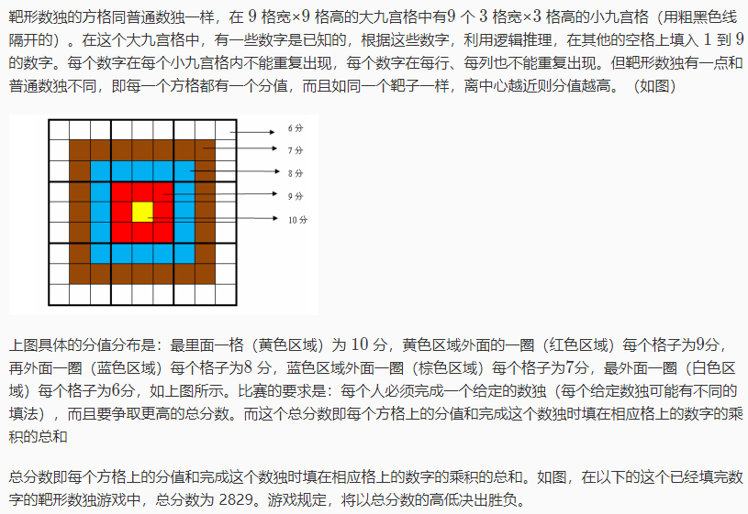
\includegraphics[width=\textwidth, height=\textheight]{luoguP1074.png}
\end{frame}

\begin{frame}{例题3——分析}
  \pause
\begin{itemize}
  \item 这道题其实更重要的并不是剪枝,而是你会不会解数独。。。 \pause
  \item 如何解数独?在前面dfs的作业就已经要求大家去学了。 \pause
  \item 如果能解数独,那么这道题就要求你快速解出权值最大的解。 \pause
  \item 这道题是有两个剪枝的: \pause
  \begin{enumerate}
  \item 在空格较少的一边开始搜,状态会比从空格多的一边搜少得多。 \pause
  \item 最优性剪枝: 设当前还没有填入的数字总和为sum, 当前的得分为cur, 最优得分为best, 如果sum*10+cur<=best, 那么已经没有继续搜索的必要了, 剪枝. (来自NOI导刊)\pause
  \end{enumerate}
\end{itemize}
\end{frame}

\begin{frame}{作业}
\begin{itemize}
  \item luoguP1092 虫食算
  \item luogu试炼场TG组的搜索Ex做绿
\end{itemize}
\end{frame}

\end{document}